\chapter{Descrição do Experimento}
\label{chap:descricao_do_experimento}

%! Escrever um pouco sobre o que é o experimento e qual o intuito

O projeto de experimentos (DOE) é um método sistemático para determinar a relação entre os fatores que afetam um processo e sua resposta ou saída. É utilizado afim de encontrar as relações de causa e efeito. Essas informações são essenciais para definir e gerenciar as entradas de um processo e otimização da resposta.

Esse trabalho tem como objetivo desenvolver um projeto de experimento com um helicóptero de papel afim de otimizar o seu tempo de voo. Para isso é necessário definir as variáveis que podem influenciar no tempo de voo como a altitude de lançamento, o tipo do papel, dimensões do corpo, dentre outras.





\section{O modelo utilizado}
\label{sec:o_modelo_utilizado}

%! Escrever sobre o helicóptero de papel e suas possíveis variáveis

O helicóptero de papel foi construído com base no modelo apresentado na Figura \ref{fig:template}.

\begin{figure}[H]
  \centering
  \caption{Modelo utilizado.}
  \includegraphics[width=0.8\textwidth]{images/template.jpeg}
  \label{fig:template}
\end{figure}


\section{As variáveis escolhidas do modelo} 
\label{sec:as_variavies_escolhidas_do_modelo}

Foram escolhidas quatro variáveis, apresentadas nas Figuras \ref{fig:f1} a \ref{fig:f6}, a serem investigadas no experimento. A altura de lançamento do helicóptero, a presença de um clipe metálico na região inferior, de um adesivo no topo ou de um adesivo lateral.

\begin{figure}[h]
    \centering
    \subfloat[2,1 metros.]{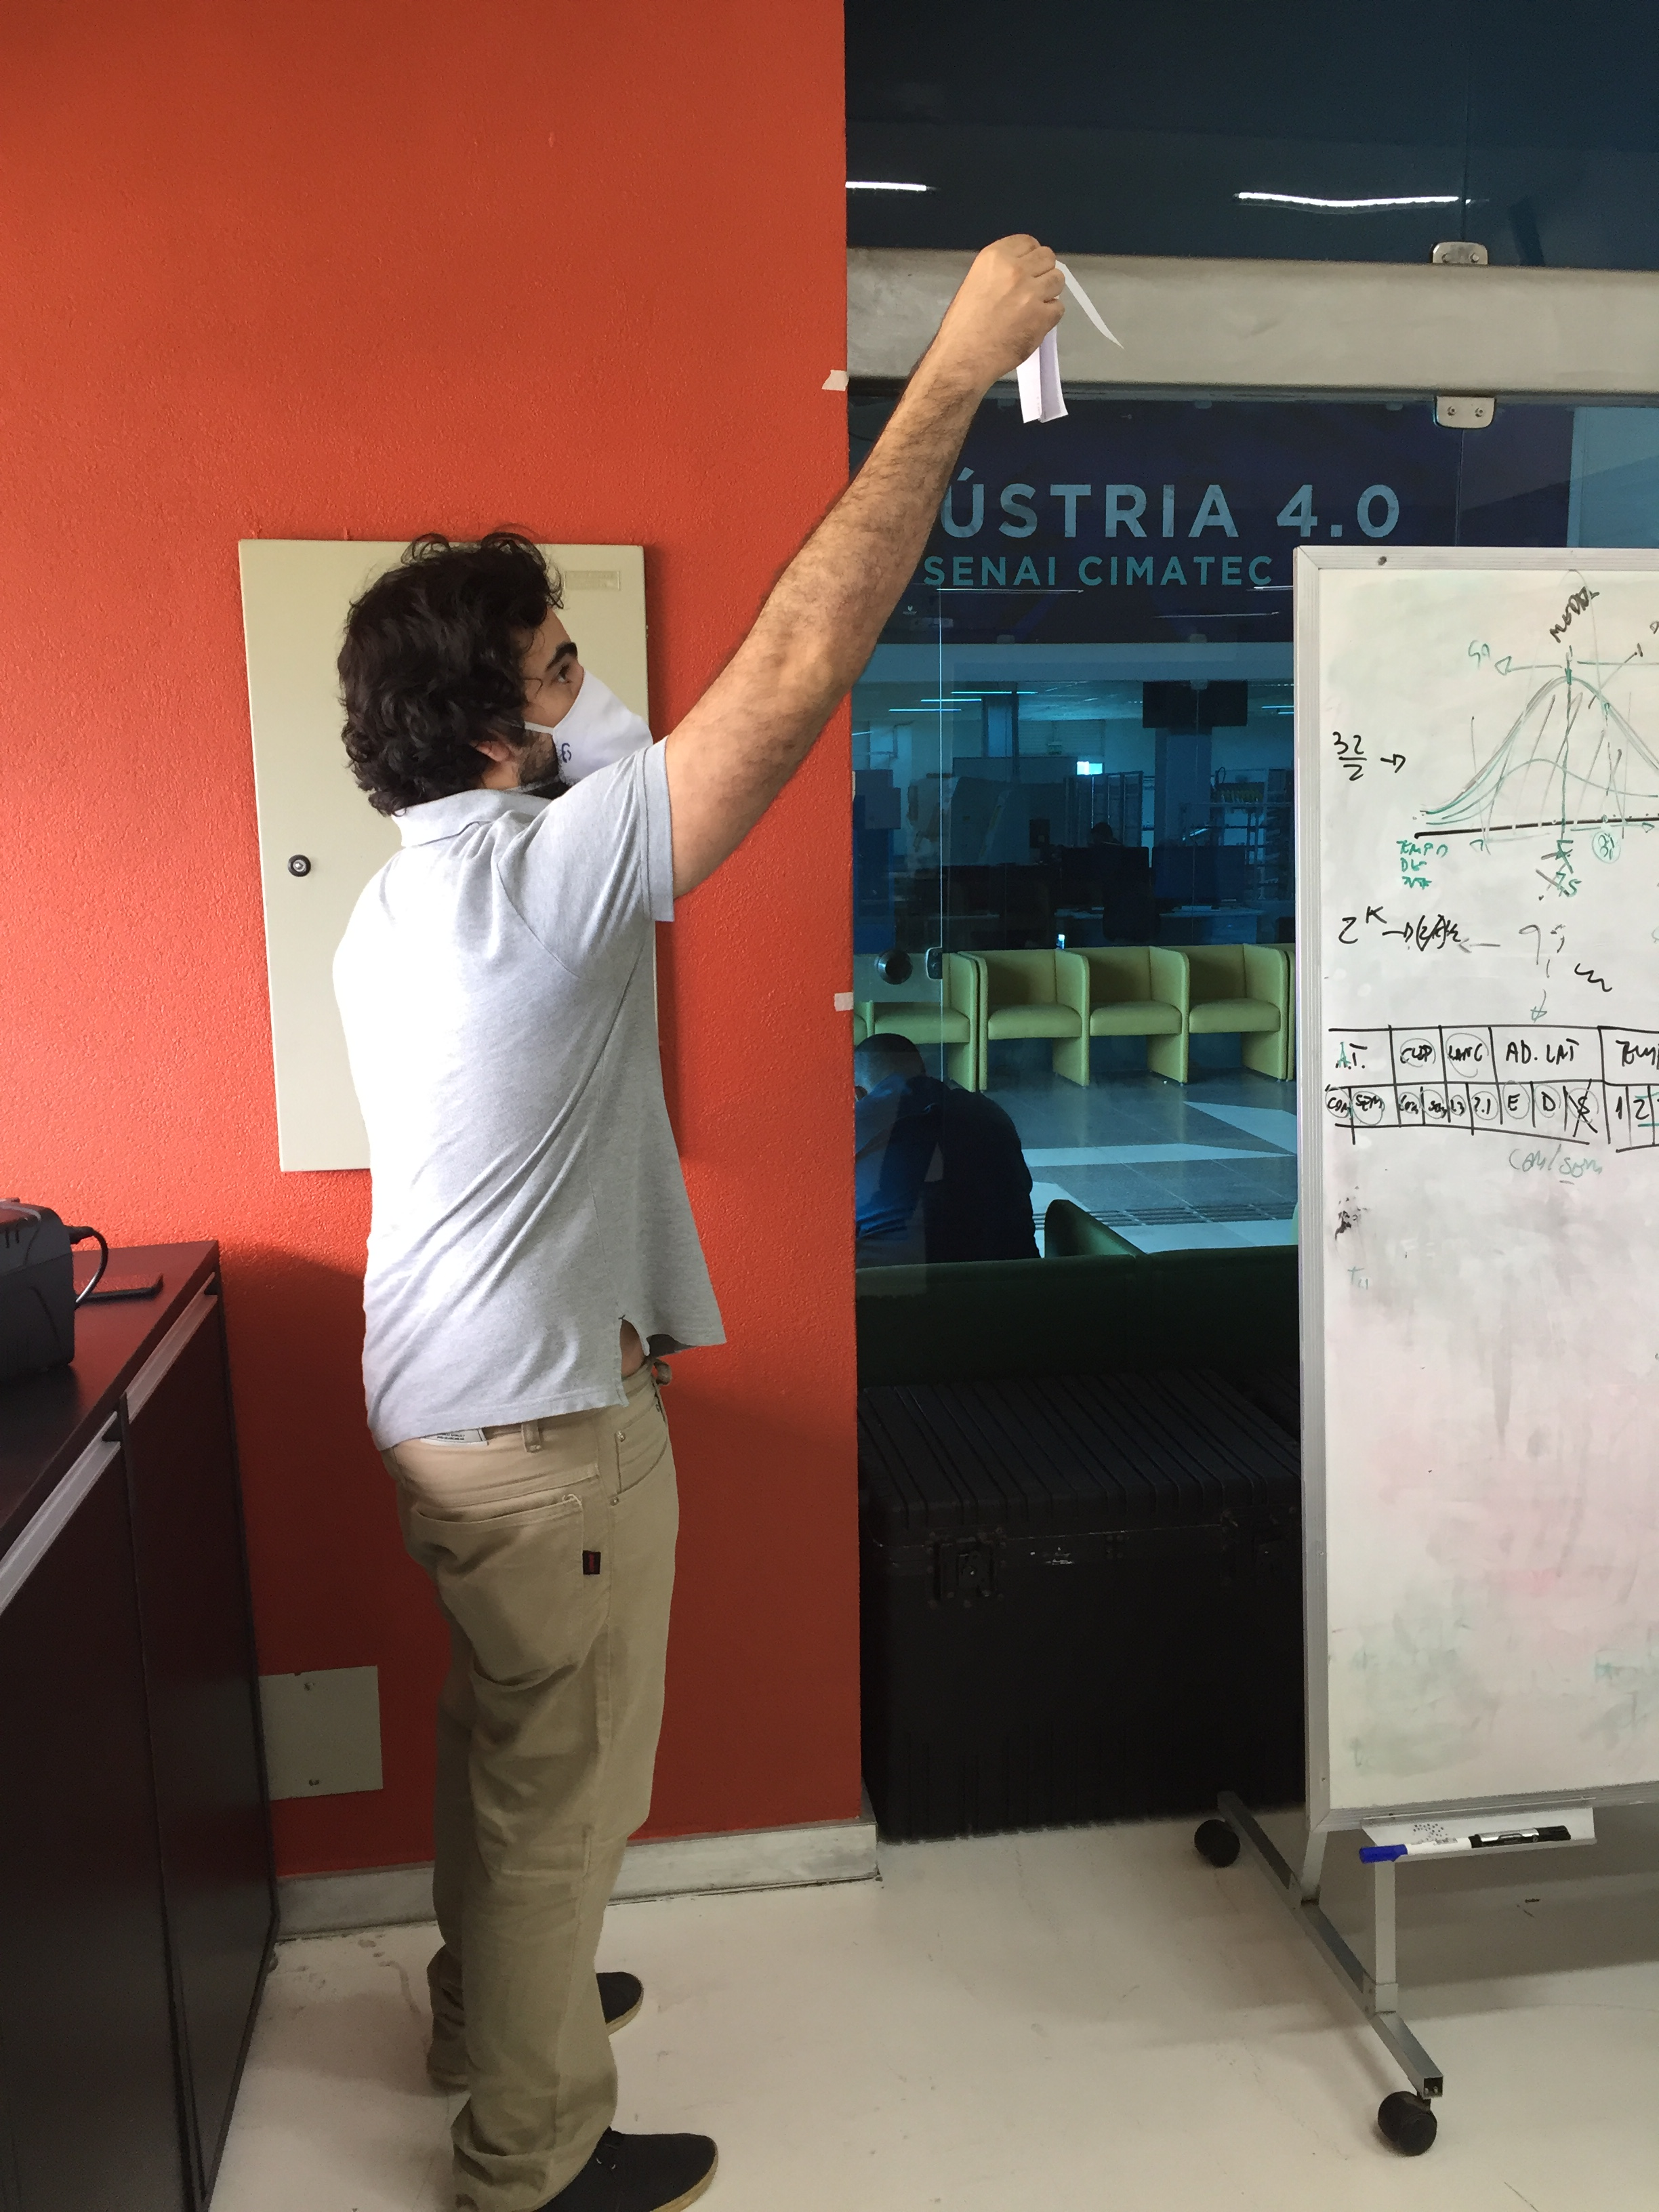
\includegraphics[width=0.4\textwidth]{images/20200909_145557439_iOS.png}\label{fig:f1}}
    \hfill
    \subfloat[1,3 metros.]{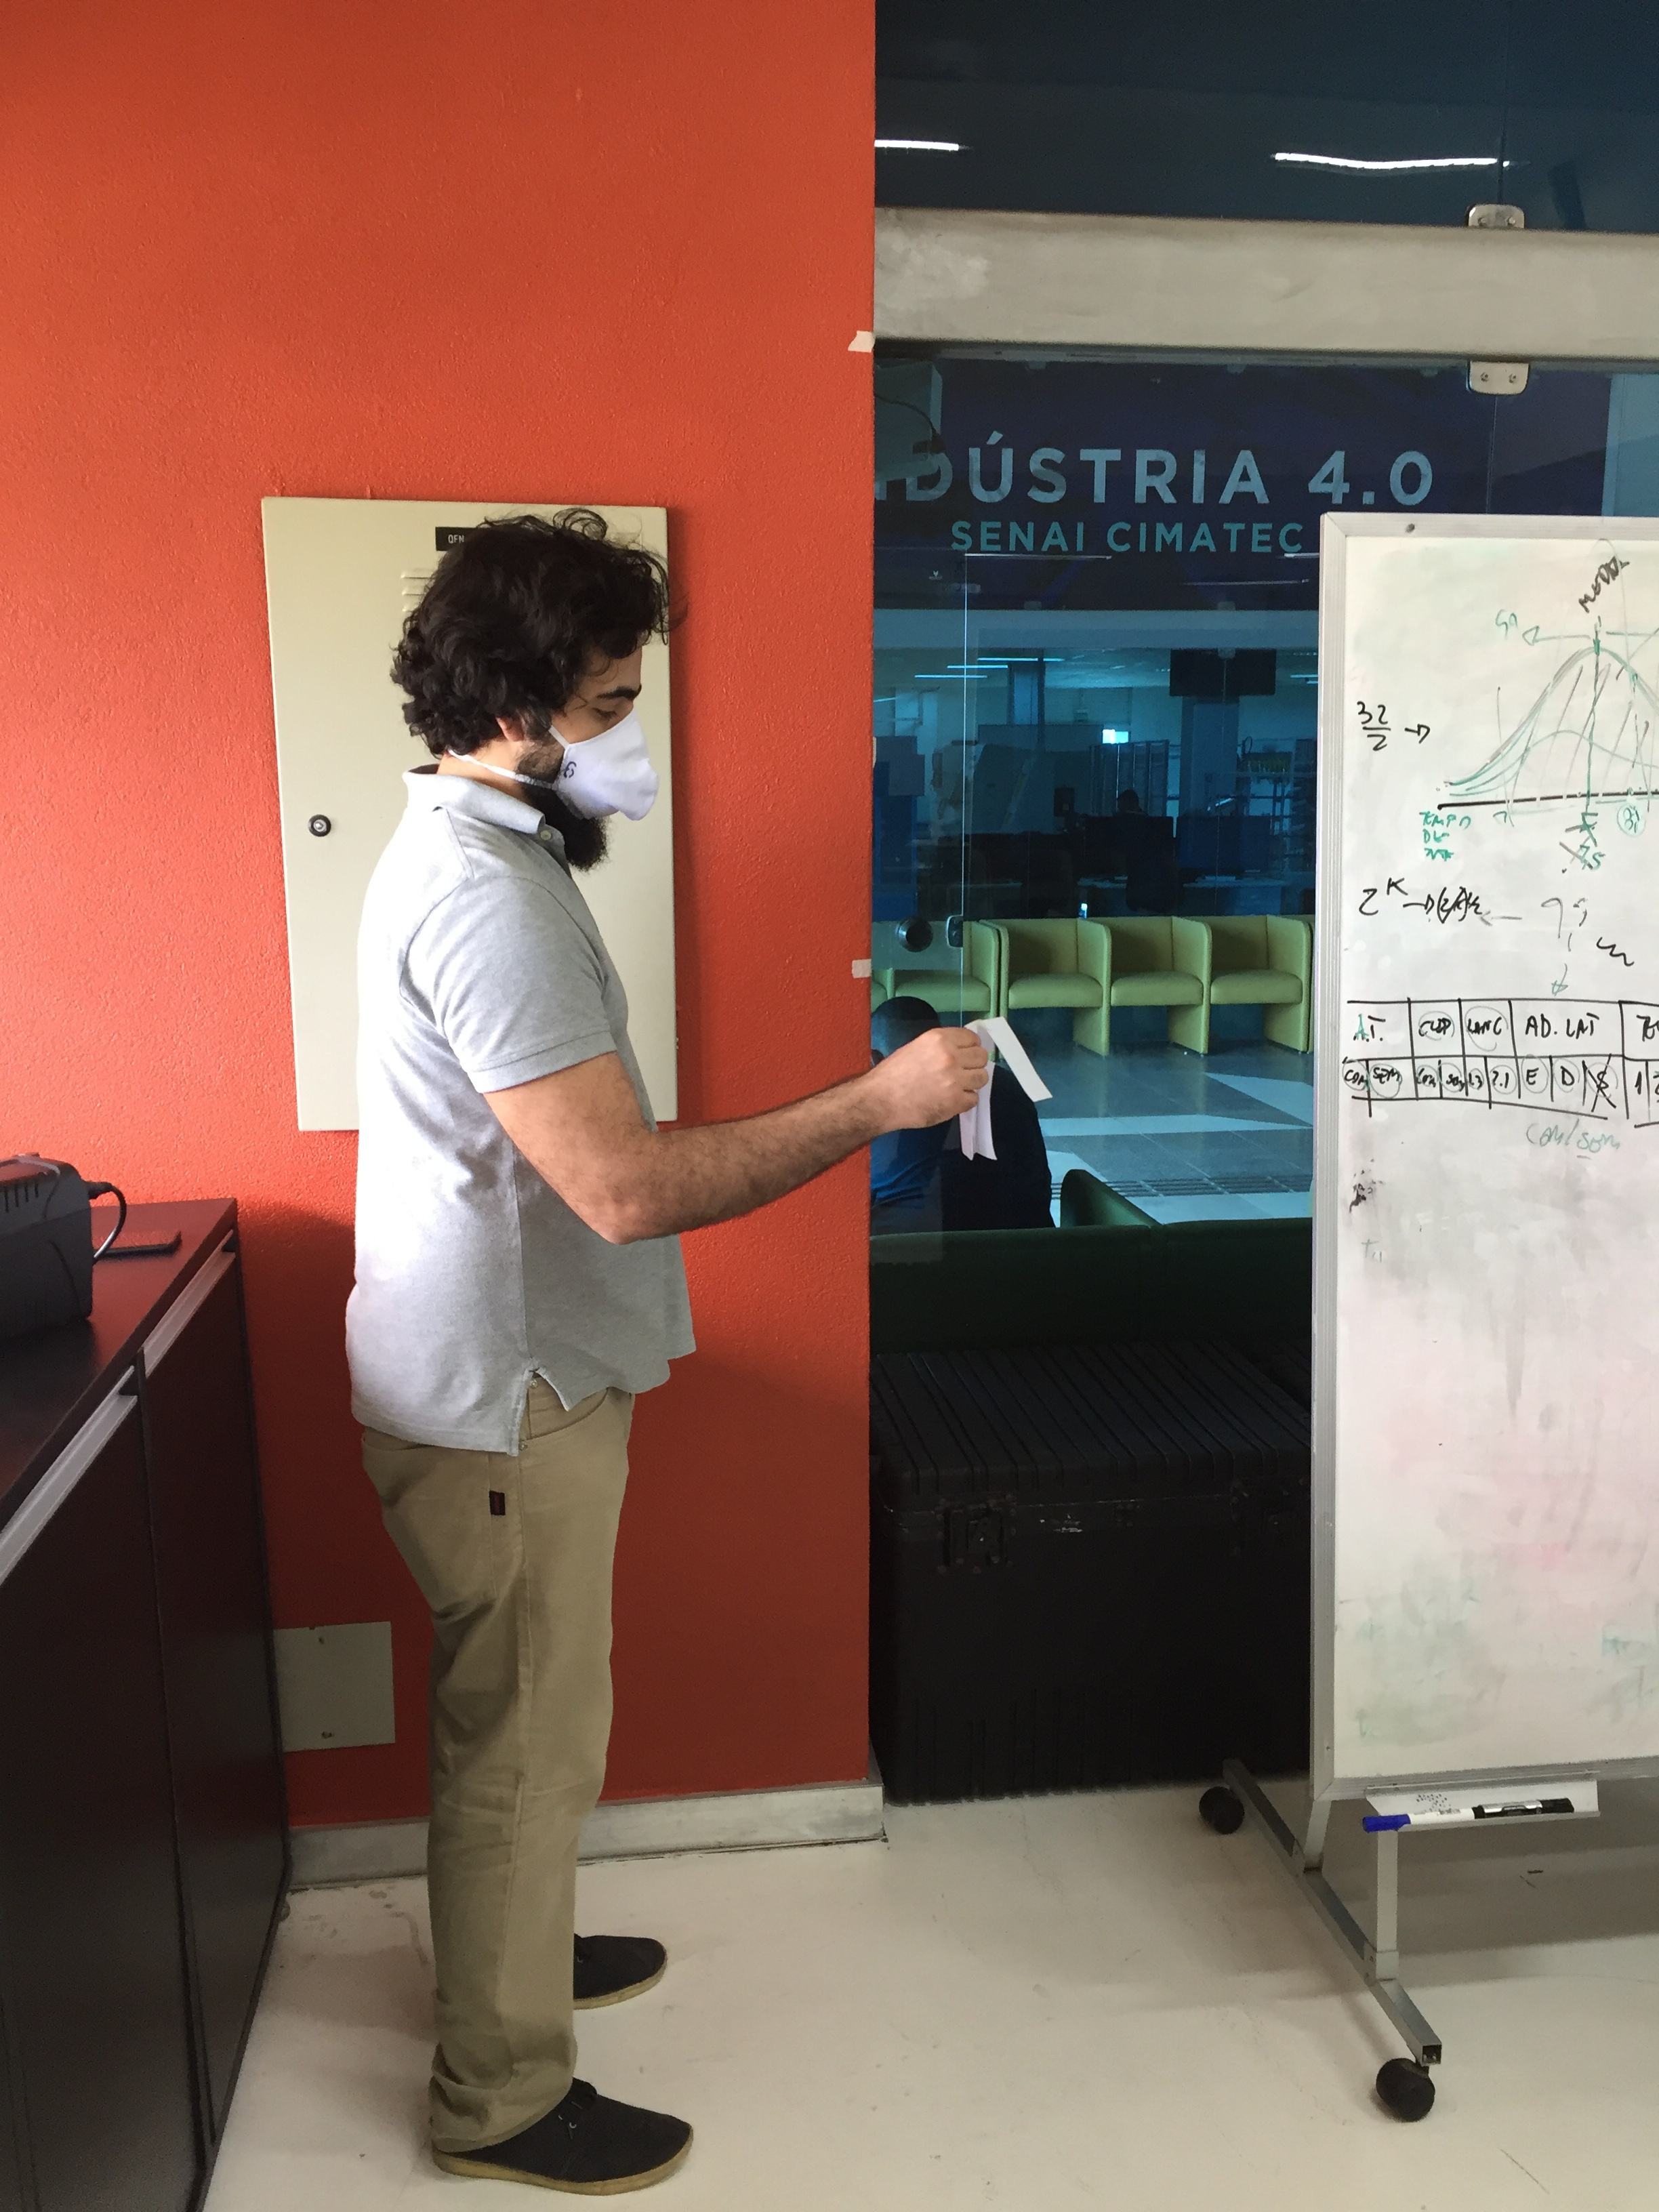
\includegraphics[width=0.4\textwidth]{images/20200909_145551403_iOS.png}\label{fig:f2}}
\caption{Altura de lançamento.}
  \end{figure}

  \begin{figure}[h]
    \centering
    \subfloat[Sem adições.]{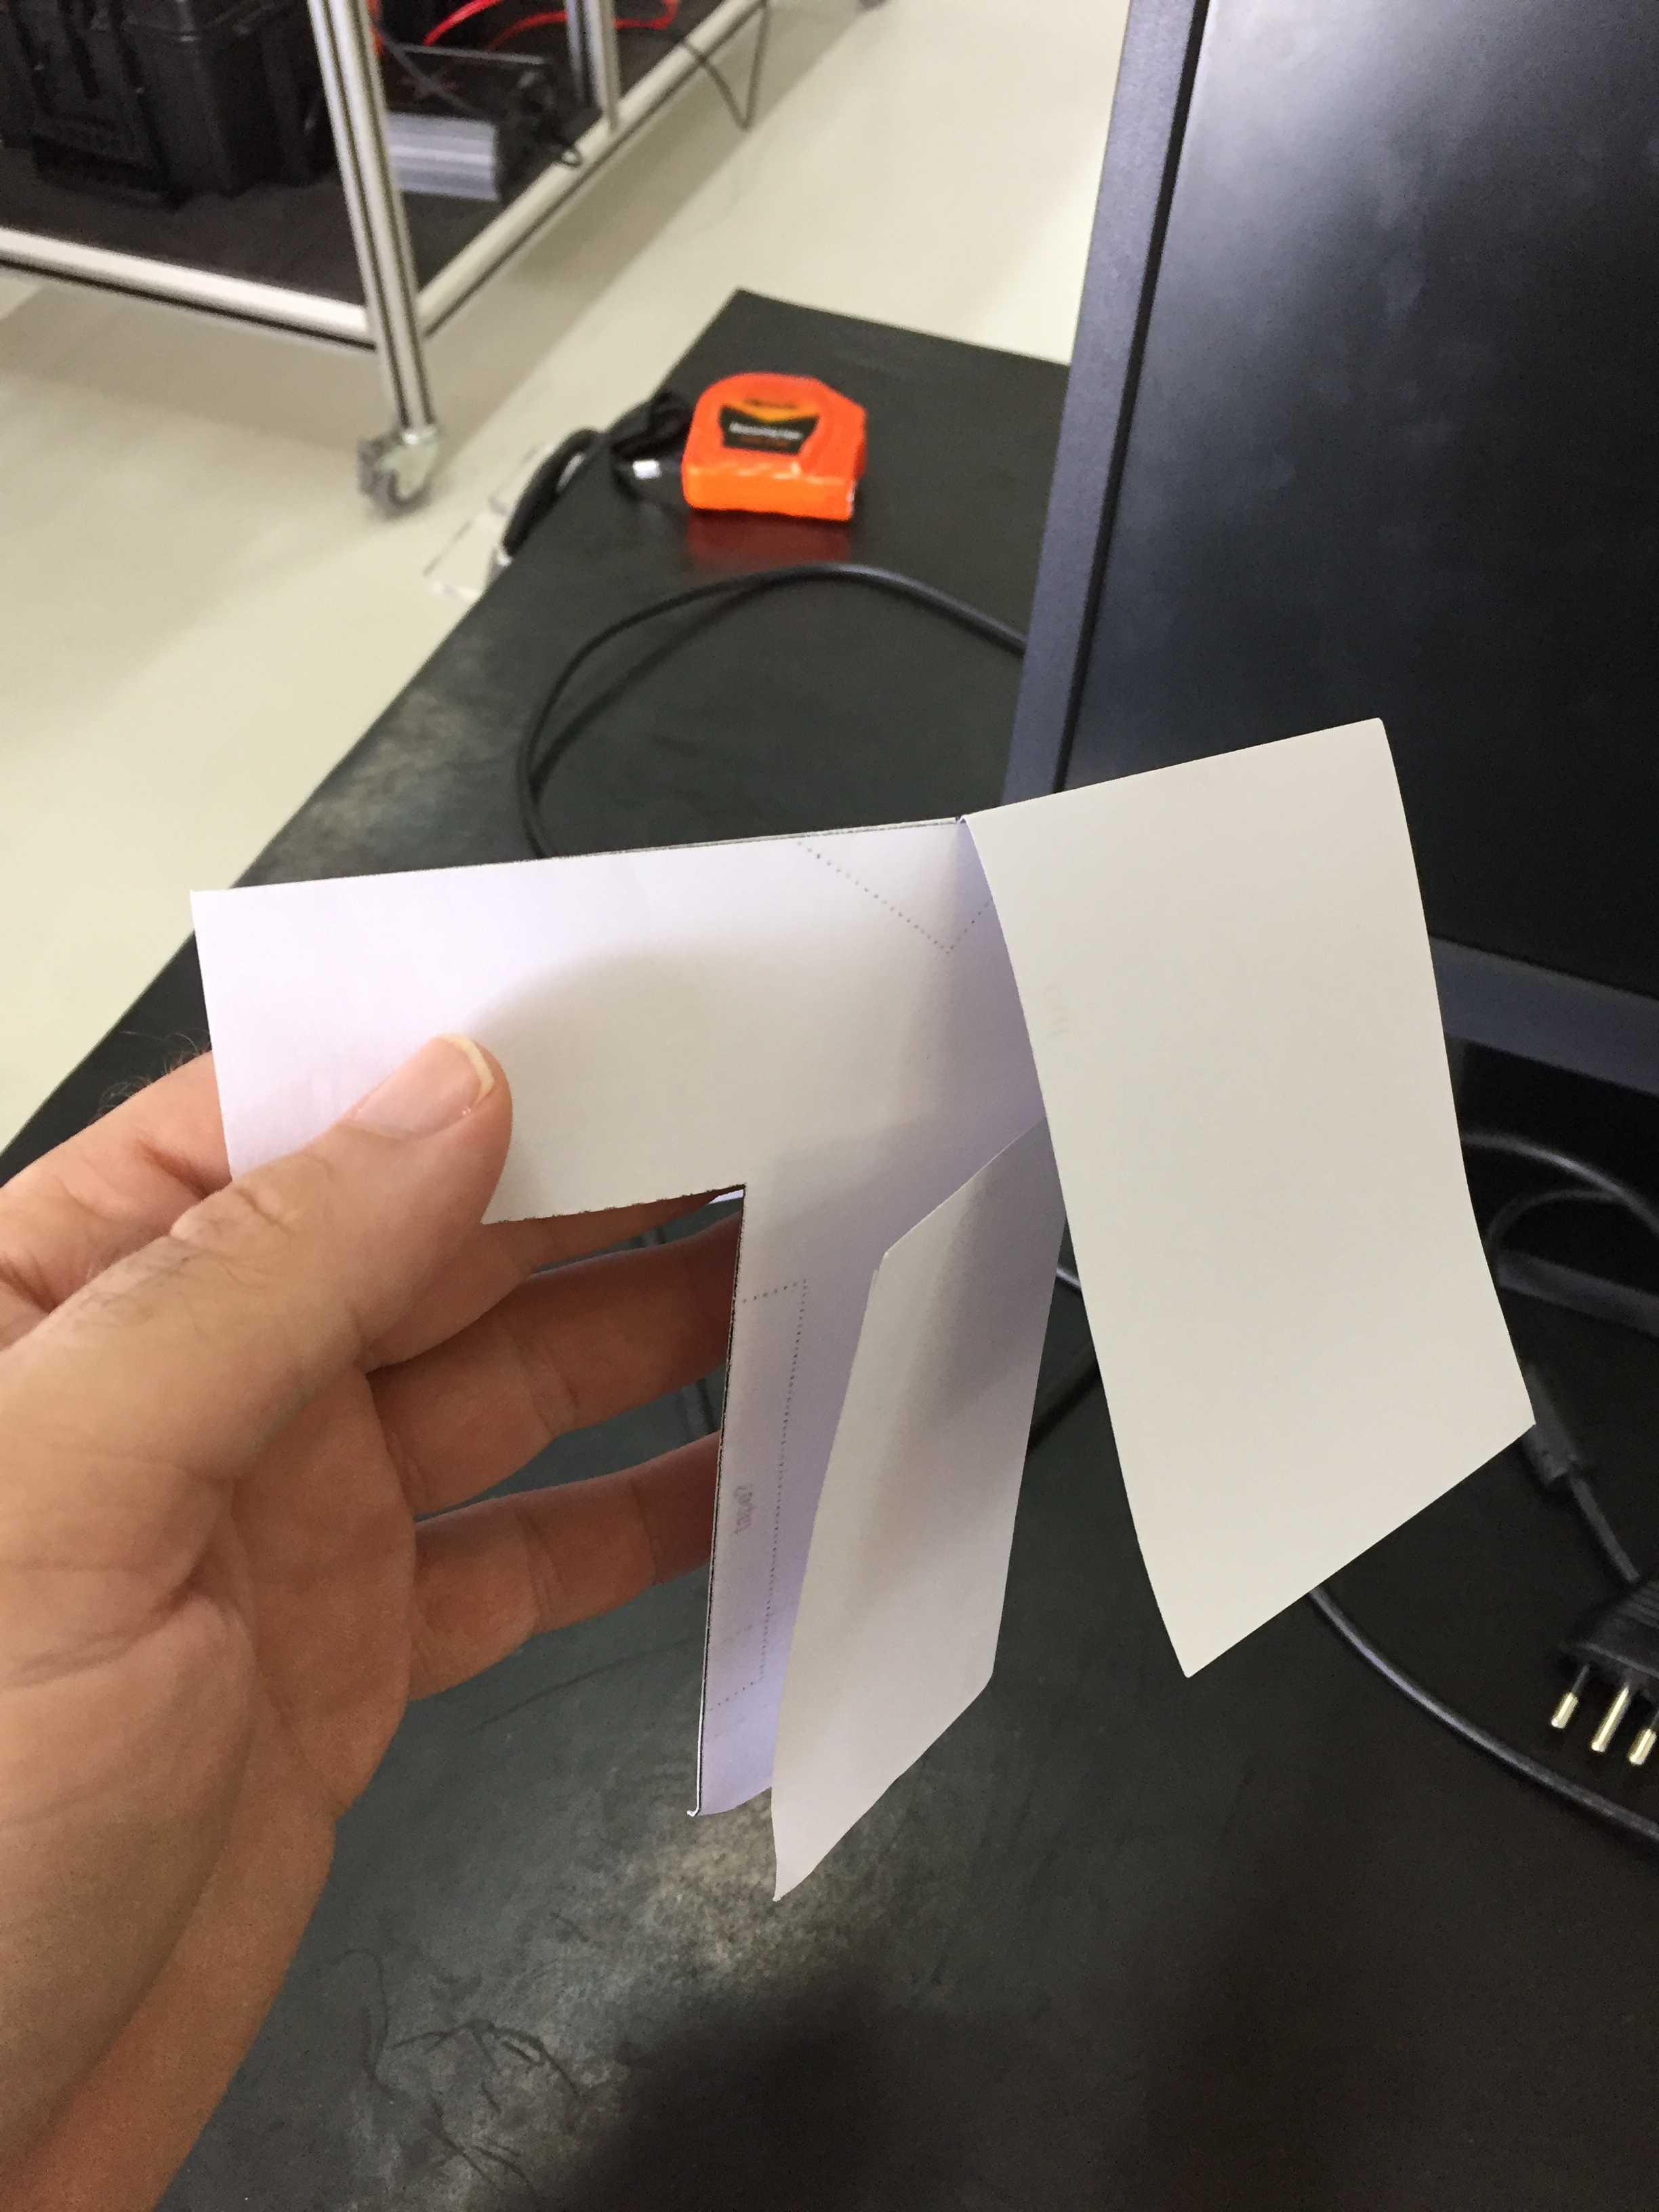
\includegraphics[width=0.4\textwidth]{images/sem_mudancas.png}\label{fig:f3}}
    \hfill
    \subfloat[Clipe na região inferior.]{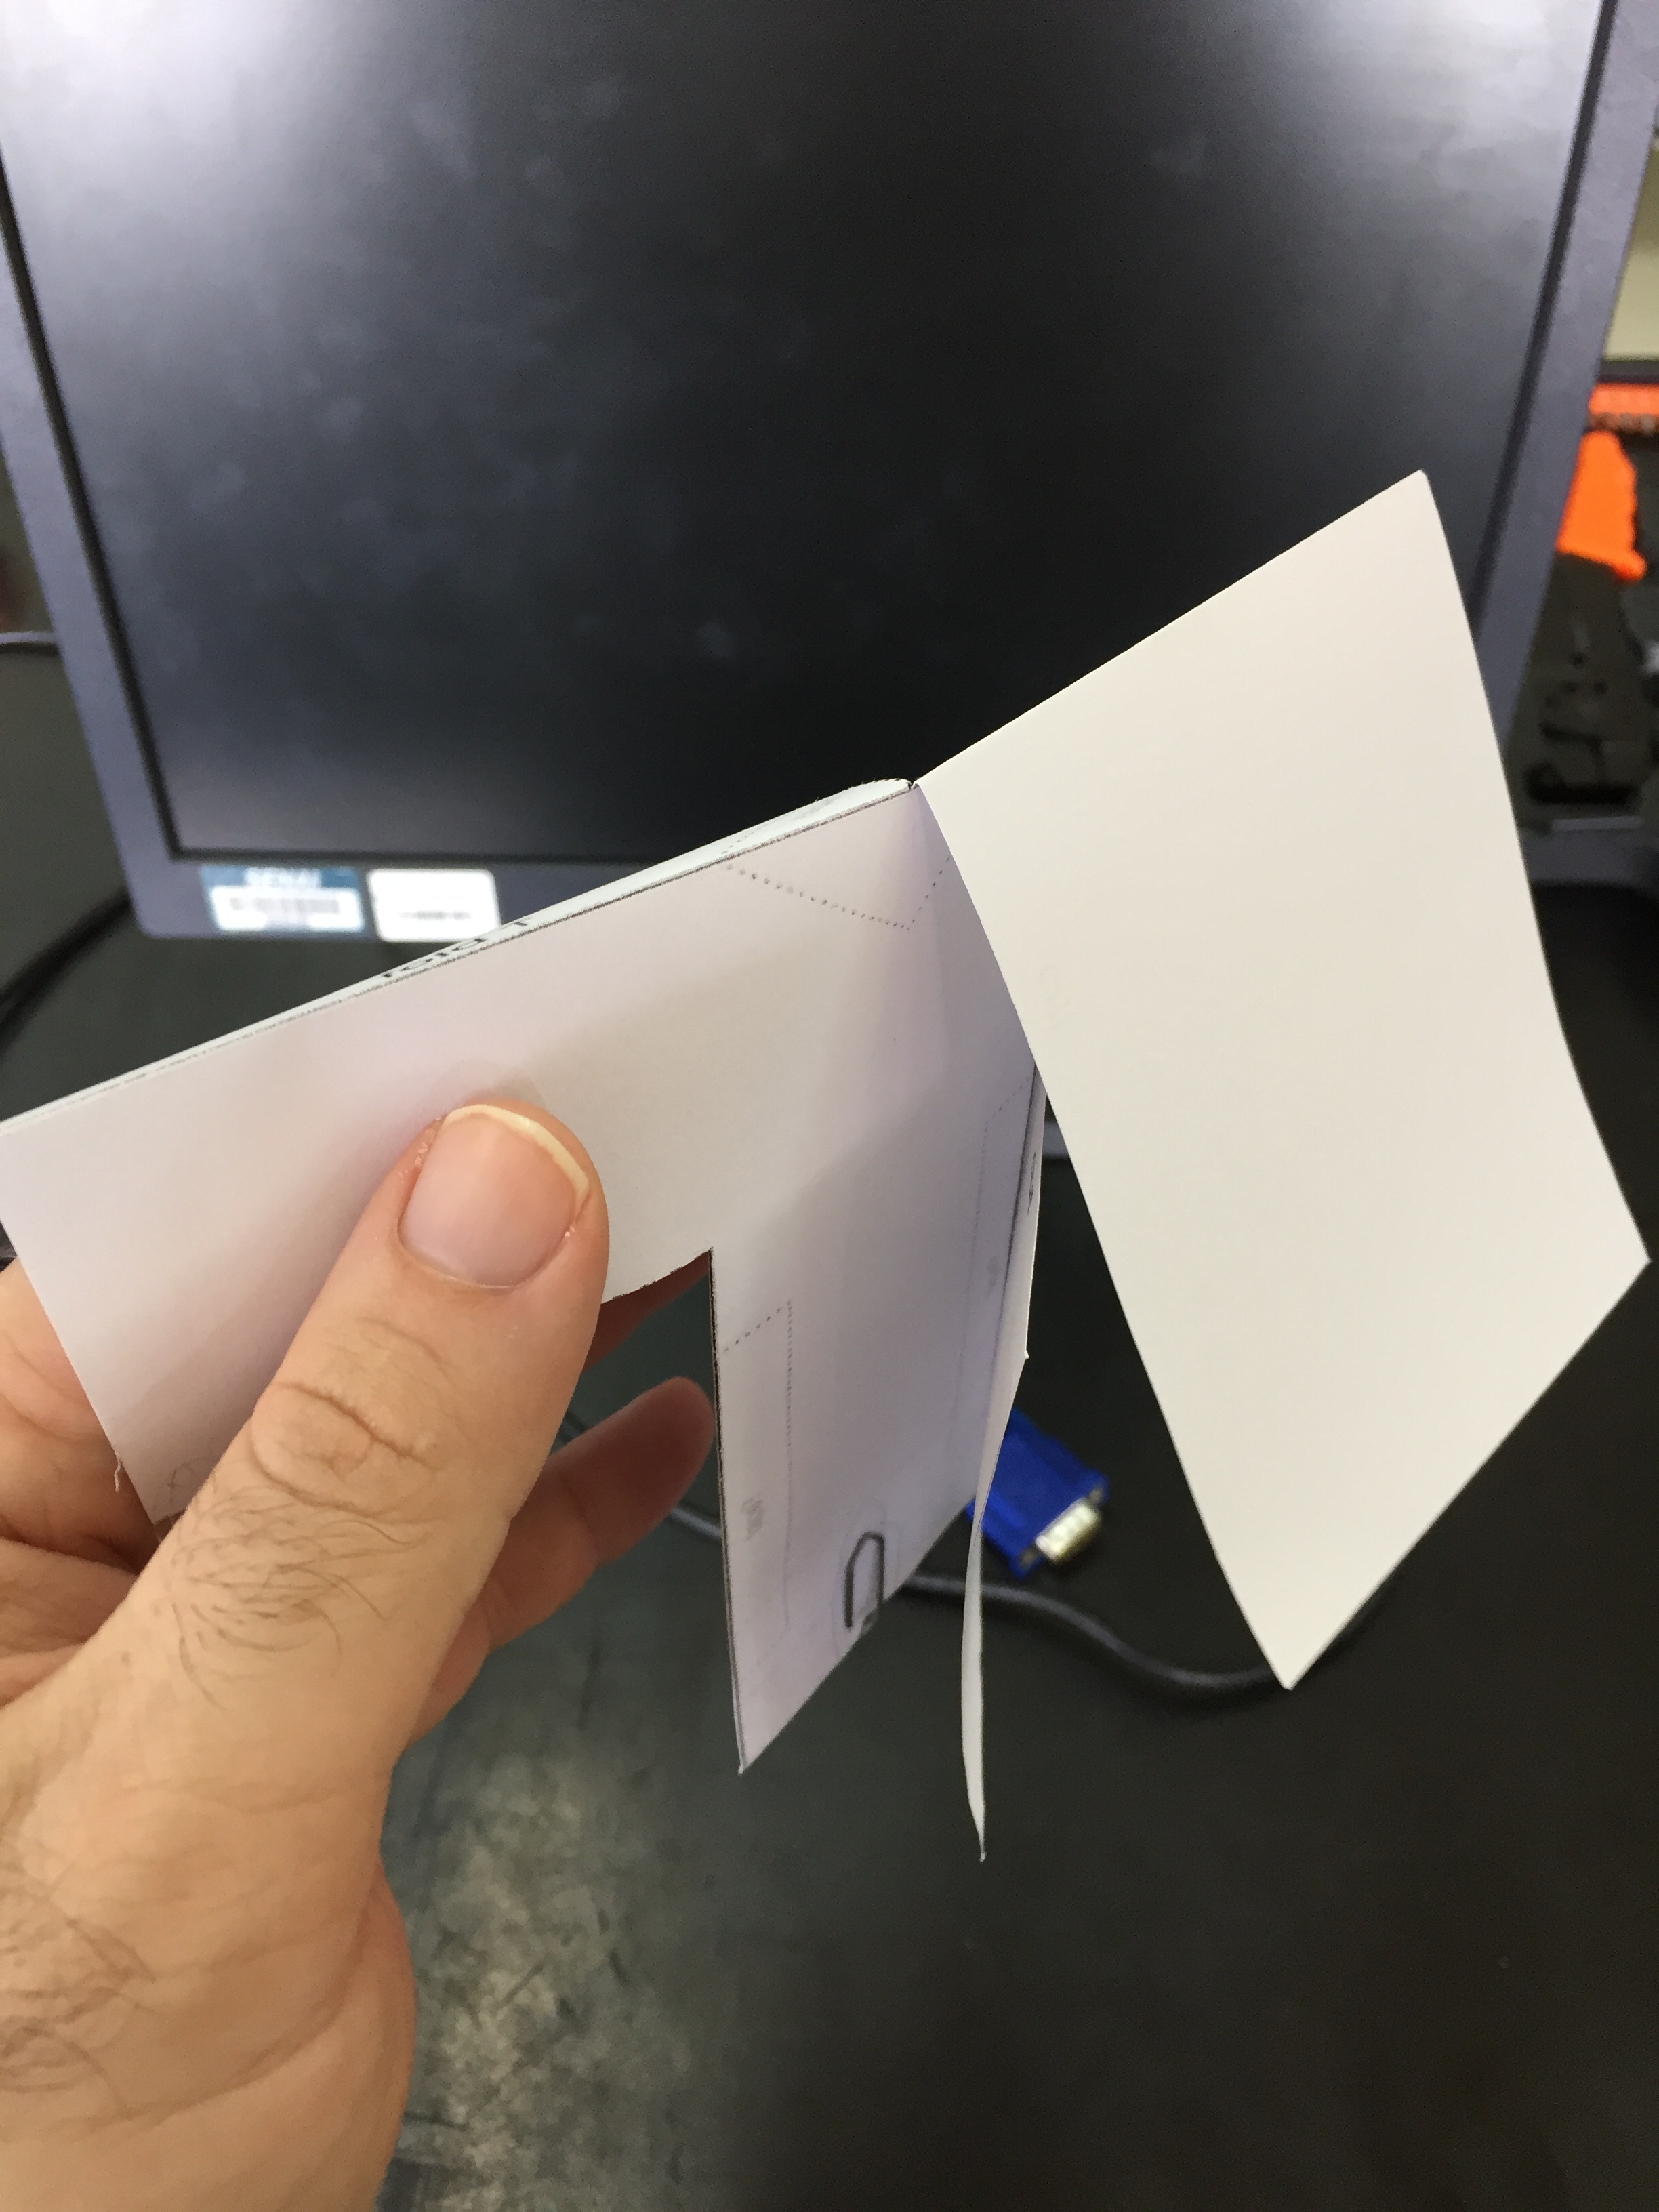
\includegraphics[width=0.4\textwidth]{images/clipe.png}\label{fig:f4}}
    \hfill
    \subfloat[Adesivo na lateral.]{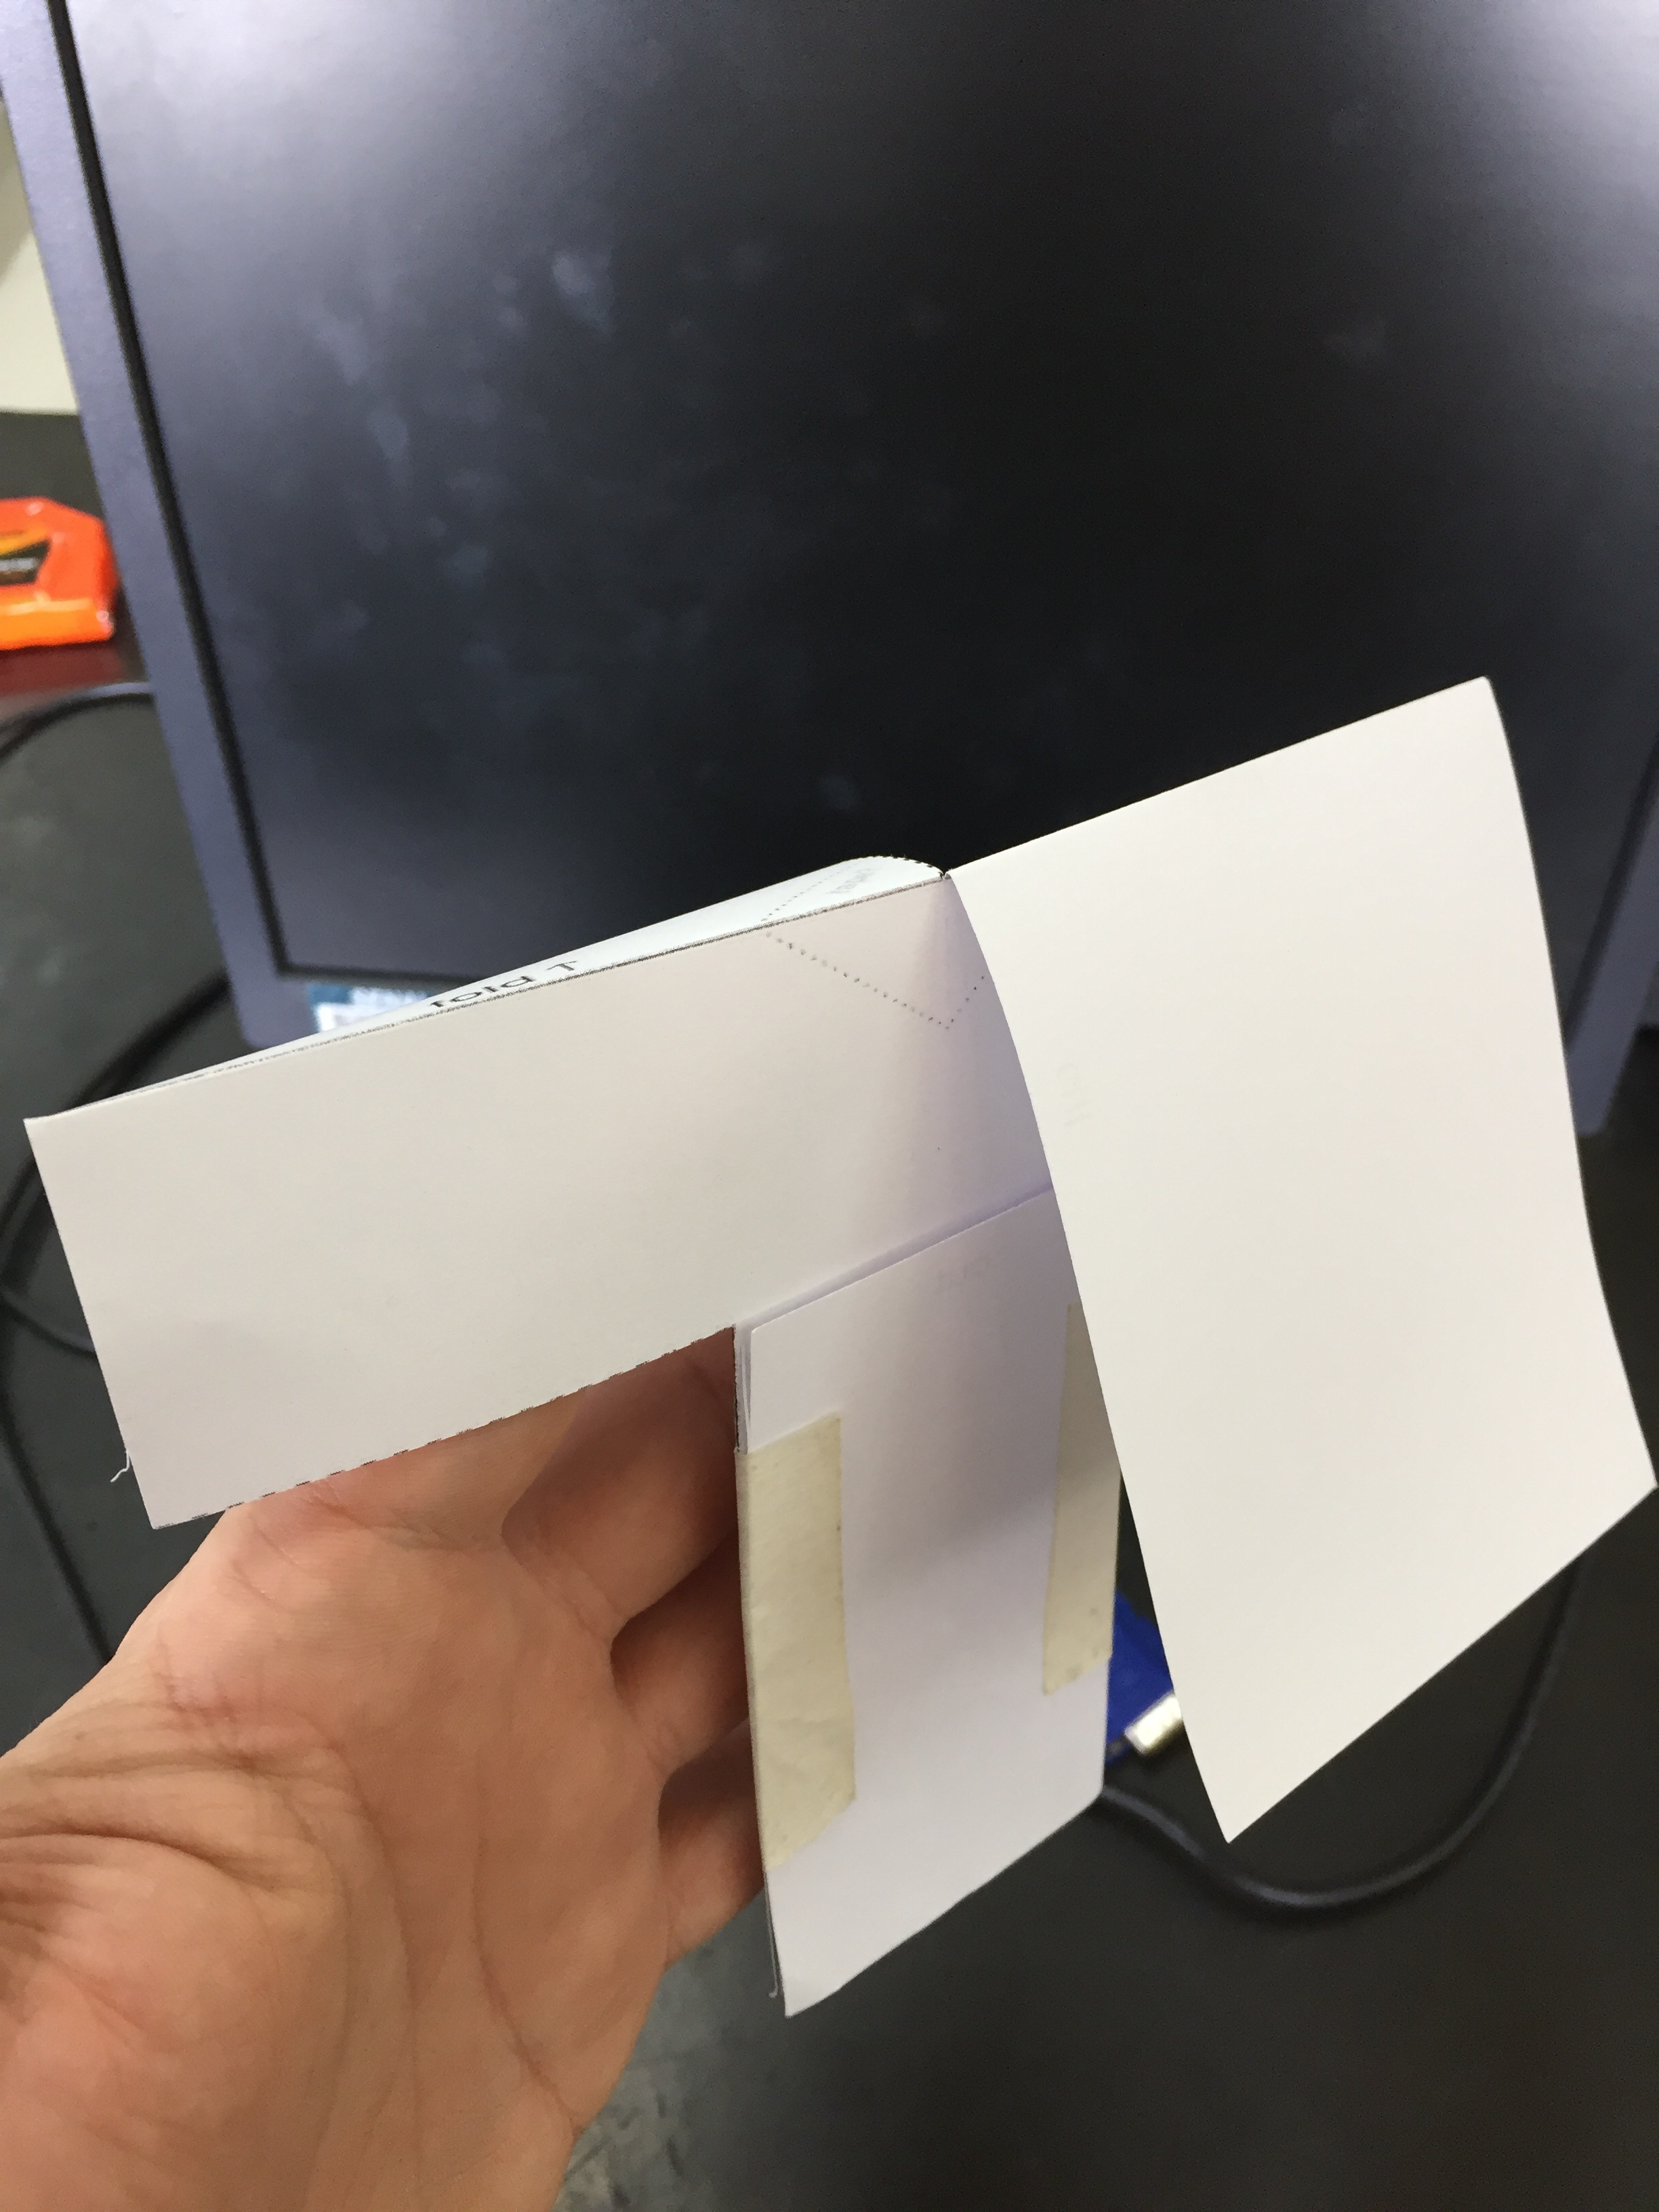
\includegraphics[width=0.4\textwidth]{images/adesivo_lateral.png}\label{fig:f5}}
    \hfill
    \subfloat[Adesivo no topo.]{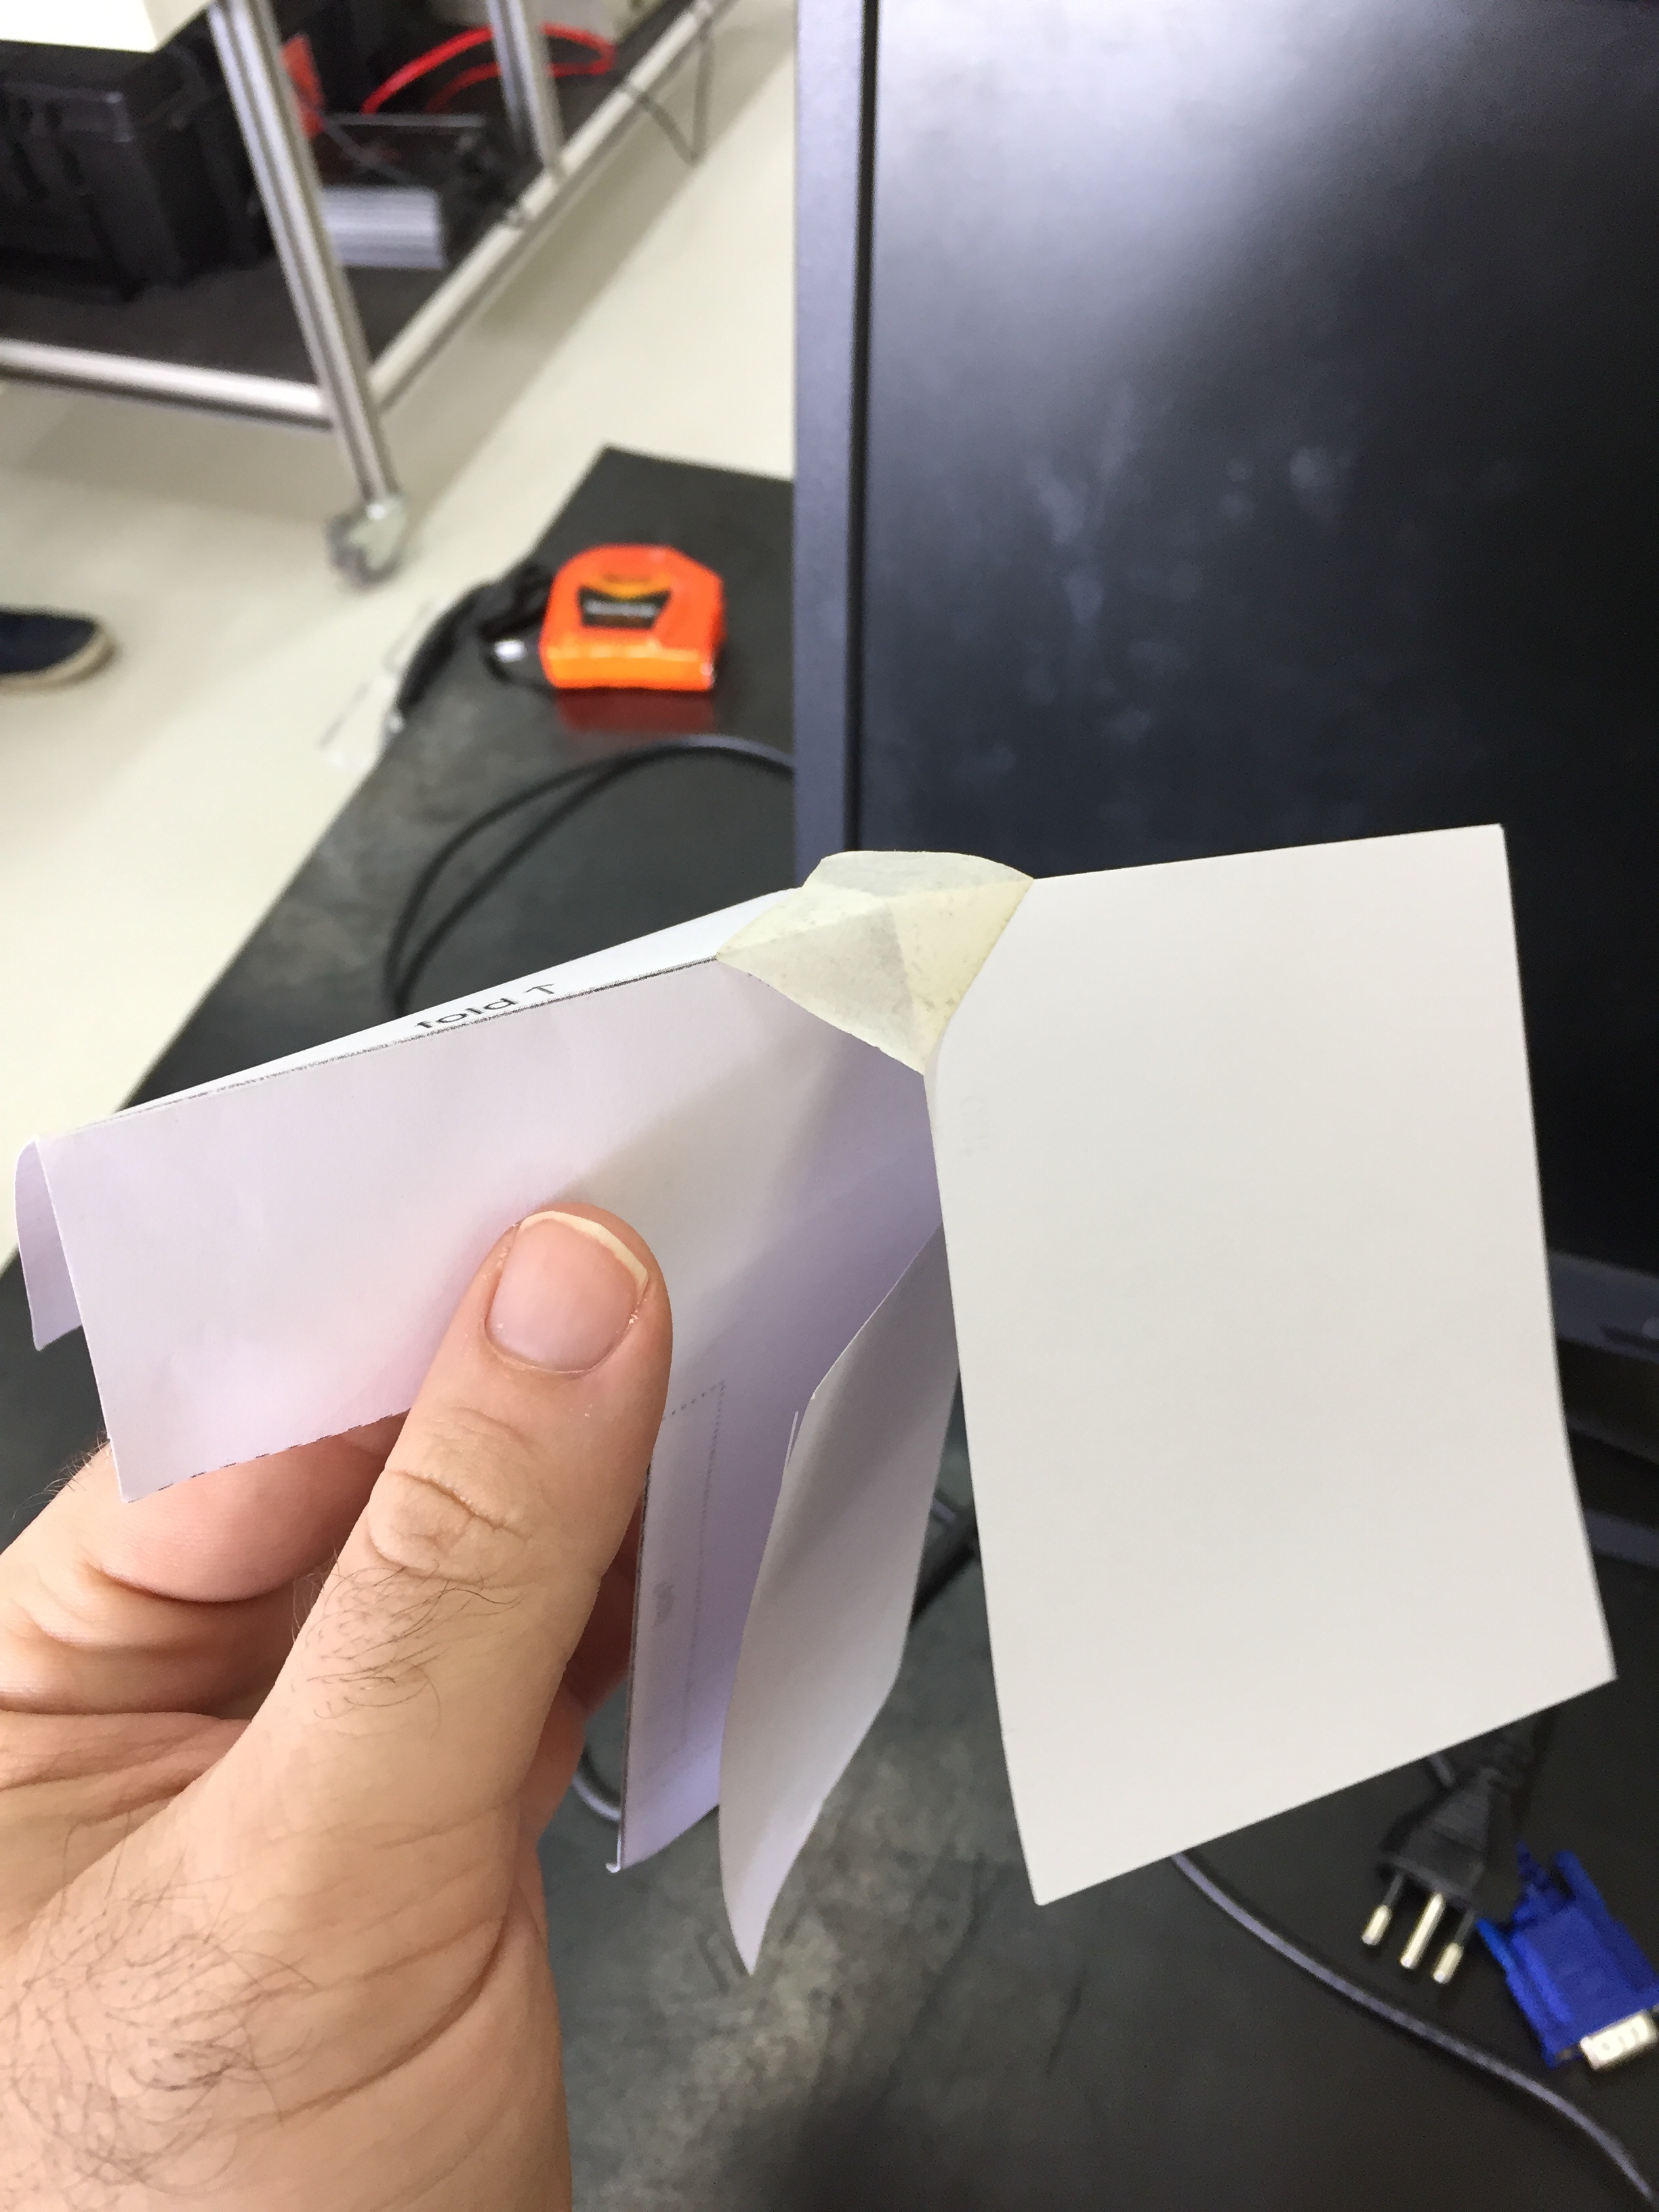
\includegraphics[width=0.4\textwidth]{images/adesivo_topo.png}\label{fig:f6}}
  \caption{Variações no corpo do helicóptero.}
  \end{figure}  

%! Escrever sobre as variáveis que foram testadas e as expectativas das suas influências -> se colocar o clipe, o peso aumenta e possivelmente o tempo de voo diminui etc...